% !TEX root = ../../../main.tex
% 来源：中学数学实验教材·第三册（高中数学）
% 章节：二次函数 / 二次函数
% 原始文件：5.tex，行 697-711
% 类型：tikz
% ---
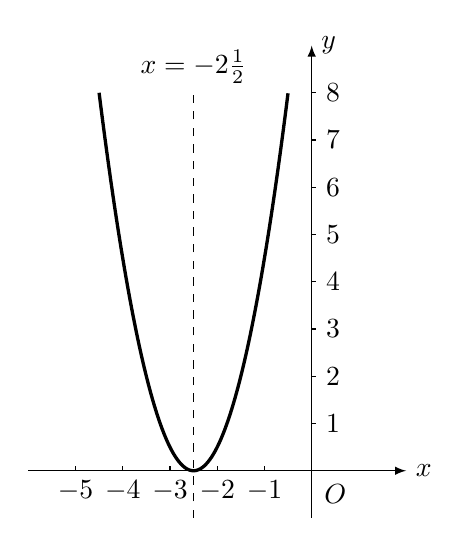
\begin{tikzpicture}[>=latex, scale=.6]
\draw[->] (-6,0)--(2,0)node[right]{$x$};
\draw[->] (0,-1)--(0,9)node[right]{$y$};
\foreach \x in {-5,-4,...,-1}
{
    \draw (\x,0)node[below]{$\x$}--(\x,.1);
}
\foreach \y in {1,2,...,8}
{
    \draw (0,\y)--(.1,\y)node[right]{$\y$};
}
\node at (.5,-.5){$O$};
\draw [domain=-4.5:-.5, samples=100, very thick]plot(\x, {2*(\x+2.5)*(\x+2.5)});
\draw[dashed](-2.5,-1)--(-2.5,8)node[above]{$x=-2\frac{1}{2}$};
\end{tikzpicture}
